% --------------------------------------------------------------
% This is all preamble stuff that you don't have to worry about.
% Head down to where it says "Start here"
% --------------------------------------------------------------
 
\documentclass[12pt]{article}
\usepackage[margin=1in]{geometry} 
\usepackage{amsmath,amsthm,amssymb}
\usepackage[margin=1in]{geometry} 
\usepackage{amsmath,amsthm,amssymb}
\usepackage[utf8]{inputenc}
\usepackage[T1]{fontenc} %escribe lo del teclado
\usepackage[utf8]{inputenc} %Reconoce algunos símbolos
\usepackage{lmodern} %optimiza algunas fuentes
\usepackage{graphicx}
\graphicspath{ {images/} }
\usepackage{hyperref} % Uso de links
\usepackage{float}
\usepackage{subfig}
\date{}


\newcommand{\N}{\mathbb{N}}
\newcommand{\Z}{\mathbb{Z}}
 
\newenvironment{theorem}[2][Theorem]{\begin{trivlist}
\item[\hskip \labelsep {\bfseries #1}\hskip \labelsep {\bfseries #2.}]}{\end{trivlist}}
\newenvironment{lemma}[2][Lemma]{\begin{trivlist}
\item[\hskip \labelsep {\bfseries #1}\hskip \labelsep {\bfseries #2.}]}{\end{trivlist}}
\newenvironment{exercise}[2][Exercise]{\begin{trivlist}
\item[\hskip \labelsep {\bfseries #1}\hskip \labelsep {\bfseries #2.}]}{\end{trivlist}}
\newenvironment{problem}[2][Problem]{\begin{trivlist}
\item[\hskip \labelsep {\bfseries #1}\hskip \labelsep {\bfseries #2.}]}{\end{trivlist}}
\newenvironment{question}[2][Question]{\begin{trivlist}
\item[\hskip \labelsep {\bfseries #1}\hskip \labelsep {\bfseries #2.}]}{\end{trivlist}}
\newenvironment{corollary}[2][Corollary]{\begin{trivlist}
\item[\hskip \labelsep {\bfseries #1}\hskip \labelsep {\bfseries #2.}]}{\end{trivlist}}

\newenvironment{solution}{\begin{proof}[Solution]}{\end{proof}}
 
\begin{document}

% --------------------------------------------------------------
%                         Start here
% --------------------------------------------------------------
 
\title{Práctica 1: Filtros de Máscaras}
\author{Víctor Manuel Arroyo Martín\\ %replace with your name
Visión por Computador}

\maketitle
\section*{Introducción}
Antes de empezar la memoria, veo necesario explicar un par de cosas:\\\\
Primero, las ejecuciones de los ejercicios 1 y 2 las he escrito a partir de la línea 483 y para ejecutar el ejercicio 3 y los bonus, por comodidad, he escrito una función para cada uno que los ejecuta por completo.\\
Segundo, he usado dos funciones auxiliares sacadas de la práctica anterior: \texttt{pintaIm} que dibuja la imagen que se le pasa por parámetro junto al nombre con el que quiere que se muestre. La otra función es \texttt{normMatrix} que normaliza una matriz, traslada sus valores al [0,1] sin pérdida de información. Esta función la uso para mostrar las imágenes con openCV, pues es necesario que estén entre [0,1].\\
También para las funciones gausssiana y sus derivadas he escrito funciones que devuelven su valor.\\
En la entrega, adjunto dentro de la carpeta "imagenes" las dos imágenes que he utilizado para hacer el bonus 2.\\
Por último, he usado la función de numpy llamada \texttt{np.pad} para añadir el relleno de reflejo y replicación a los bordes de la imagen.

\section*{Ejercicio 1}

\subsection*{Apartado 1.A}

Para este primer apartado he creado la función \texttt{gaussianMask1D} que crea una máscara gaussiana discretizada de una dimensión tomando en el intervalo [-3$\sigma$, 3$\sigma$+1] (95$\%$ del área bajo la función) todos los enteros, que serán en total 3*2*$\sigma$+1, aplicándoles la gaussiana a todos y normalizándolos.\\
De la misma forma, he creado las máscaras derivadas con \texttt{derivGaussianMask1D} pero en vez de aplicar la gaussiana a cada entero, se aplica la derivada de la gaussiana correspondiente (la primera o segunda según se indique por parámetro).\\\\
También he creado una función para aplicar una máscara 1D a un vector y comprobar así el funcionamiento de las funciones anteriormente descritas. Llamada \texttt{apply1DMask}, convoluciona una máscara 1D con un vector con tres posibles modos de borde: con ceros, con reflejo y con replicación (el reflejo y la replicación se usarán en los siguientes ejercicios). Para convolucionar he hecho dos bucles que ejecutan lo explicado en teoría para la correlación (la convolución es solo dar la vulta a la máscara): G = H $\otimes$ F.\\
Las funciones las compruebo mediante la creación de un vector con valores aleatorios y apliándole las máscaras gaussiana y sus derivadas con $\sigma$=2, así como mostrando la gráfica de las funciones gaussiana y derivadas y comprobar que efectivamente están bien.

\begin{figure}[H]
\centering
\parbox{7cm}{
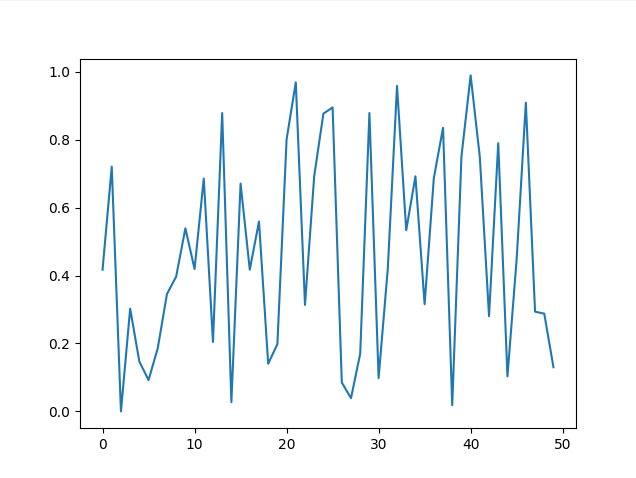
\includegraphics[width=7cm]{images/VectorAleat.png}
\caption{Vector aleatorio representado.}
\label{fig:2figsA}}
\qquad
\begin{minipage}{7cm}
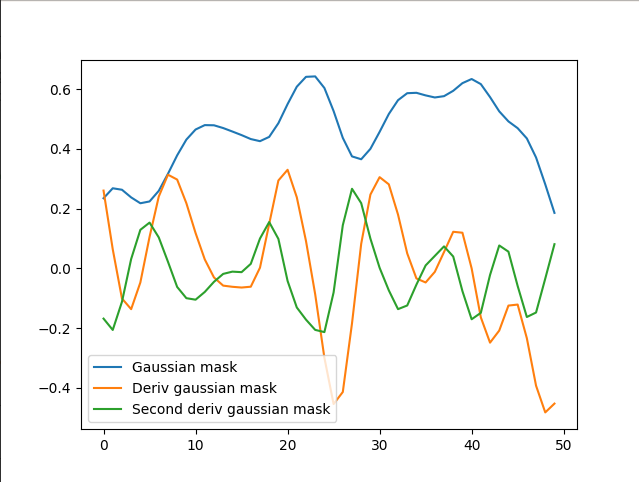
\includegraphics[width=7cm]{images/VectorAleatMask.png}
\caption{Máscaras aplicadas al vector.}
\label{fig:2figsB}
\end{minipage}
\end{figure}

Como se ve en estas dos figuras, se pasa de un vector aleatorio, a una función más suavizada gracias a aplicar las máscaras gaussianas. Ahora, para terminar de comprobar que se han realizado bien las máscaras veamos su representación en una gráfica.

\begin{figure}[H]
\centering
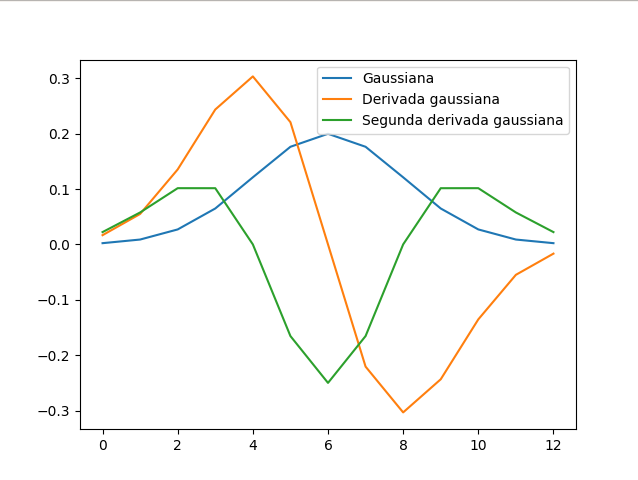
\includegraphics[scale=0.45]{images/GaussianMask.png} 
\caption{Máscara gaussiana y sus derivadas.}
\label{etiqueta}
\end{figure}

La forma de las funciones a simple vista se ve que son correctas: la gaussiana tiene forma de sombrero y sus derivadas también tienen la forma que deberían tener.

\subsection*{Apartado 1.B}

En esta sección he creado una función llamada \texttt{applySeparable2DMask} a la que se le pasan los dos vectores en los que se separa una matriz 2D separable y aplica por filas y por columnas con \texttt{apply1DMask} las dos máscaras. Tiene tres modos de borde: con reflejo, con ceros y con réplica y diferencia entre las imágenes de color y de escalas de grises. Para una imagen en color, se aplica la máscara gaussiana en cada canal de color y para una imagen de grises, directamente.\\\\
En la ejecución de este ejercicio, he usado la imagen del gato para probar las máscaras con un $\sigma$ = 2 y 4 y el modo de borde "cero" y "reflect" para rellenarlo. Por último, para comparar con la función de openCV \texttt{GaussianBlur}, he pasado por parámetros a ésta el tamaño de la máscara gaussiana que calculé para aplicarla a la imagen del gato y el mismo valor de $\sigma$. Los resultados son los siguientes tanto en color como en blanco y negro:\\

\begin{figure}[H]
\centering
\parbox{4cm}{
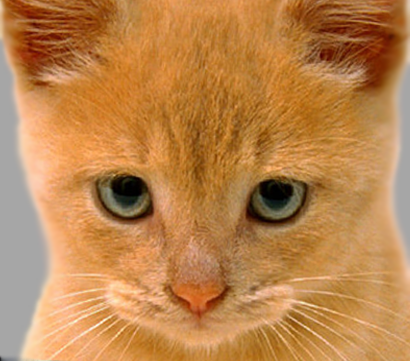
\includegraphics[width=4cm]{images/OriginalCat.png}
\caption{Imagen original a color.}
\label{fig:2figsA}}
\qquad
\begin{minipage}{4cm}
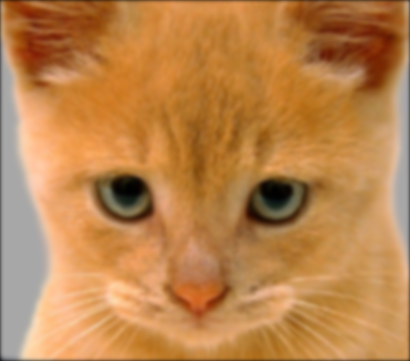
\includegraphics[width=4cm]{images/GaussianCat.png}
\caption{Imagen con el filtro gaussiano $\sigma$=2.}
\label{fig:2figsB}
\end{minipage}
\qquad
\begin{minipage}{4cm}
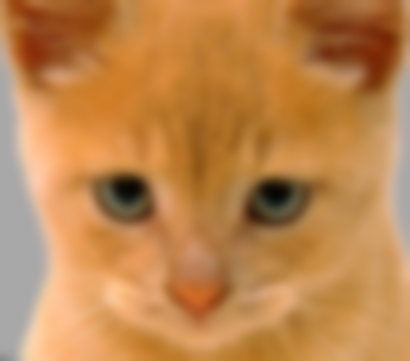
\includegraphics[width=4cm]{images/GaussianCatBigSigma.png}
\caption{Imagen con filtro gaussiano con $\sigma$=4.}
\label{fig:2figsB}
\end{minipage}
\end{figure}

Como se ve en la segunda imagen, queda ligeramente más borrosa que la original pues sigma=2 es bajo, los colores se amortiguan y los bordes son negros por haberlos rellenado con ceros. Para la imagen con sigma=4 se aprecia un desenfoque o borrosidad mucha mayor y el modo de borde seleccionado ha sido reflejo así que no aparecen los bordes negros de la otra imagen. Ahora veamos las máscaras derivadas de la imagen a color:\\
\begin{figure}[H]
\centering
\parbox{5cm}{
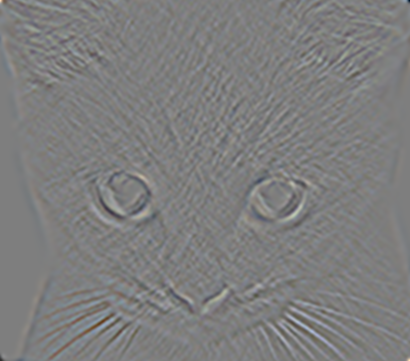
\includegraphics[width=5cm]{images/GaussianCatDeriv.png}
\caption{Máscara gaussiana primera derivada.}
\label{fig:2figsA}}
\qquad
\begin{minipage}{5cm}
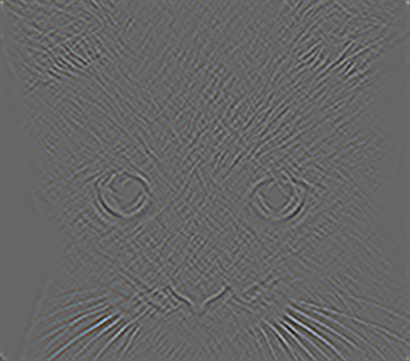
\includegraphics[width=5cm]{images/GaussianCatDeriv2.png}
\caption{Máscara gaussiana segunda derivada.}
\label{fig:2figsB}
\end{minipage}
\end{figure}

Vemos que los bordes de las siluetas de la imagen se realzan pues hay cambio brusco de color. Por último comparamos \texttt{gaussianBlur} en blanco y negro con nuestro filtro.\\
\begin{figure}[H]
\centering
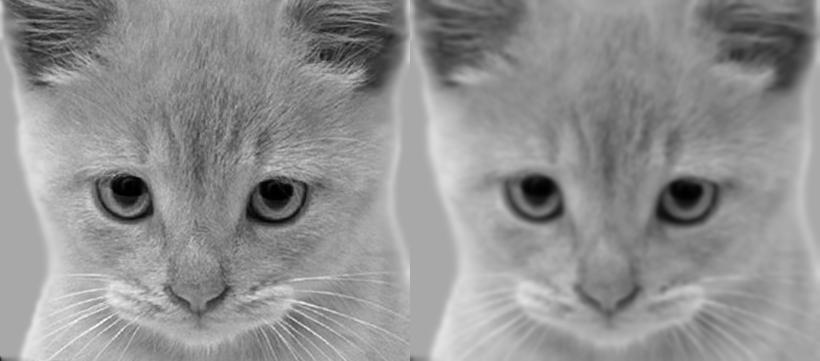
\includegraphics[scale=0.45]{images/GaussianCatBlur.png} 
\caption{Imagen generada por \texttt{gaussianBlur}.}
\label{etiqueta}
\end{figure}
\begin{figure}[H]
\centering
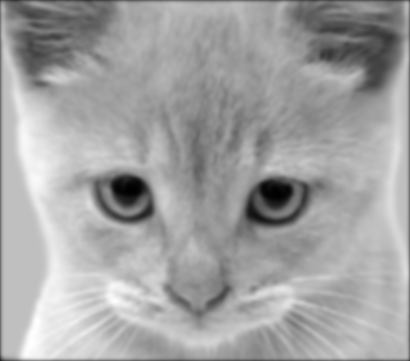
\includegraphics[scale=0.45]{images/GaussianCatBW.png} 
\caption{Imagen con filtro gaussiano en blanco y negro.}
\label{etiqueta}
\end{figure}
Como podemos ver a penas se diferencian, excepto en los bordes pues en nuestro algoritmo se usan los bordes negros. Nuestra imagen es más clara pues los bordes negros afectan a la imagen al completo.

\subsection*{Apartado 1.C}
Para este apartado he investigado un poco sobre la función de openCV \texttt{getDerivKernels} para ver las diferencias con la máscara gaussiana que se ha calculado en esta práctica y he encontrado que la diferencia se halla en que en vez de calcular un kernel gaussiano, calcula un kernel sobel que a pesar de tener la misma forma al representarla, no es un filtro gaussiano como tal. A continuación pongo los ejemplos que he pintado para comprobarlo.\\
Primero, las gráficas de las funciones:
\begin{figure}[H]
\centering
\parbox{7cm}{
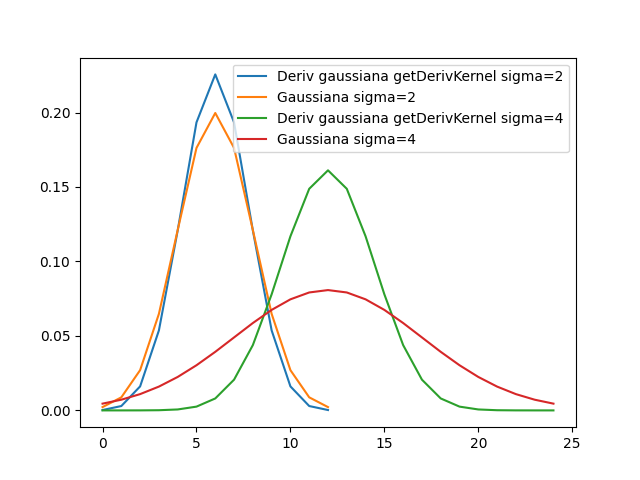
\includegraphics[width=7cm]{images/GaussianaGetDerivKernels.png}
\caption{Máscaras sin derivar.}
\label{fig:2figsA}}
\qquad
\begin{minipage}{7cm}
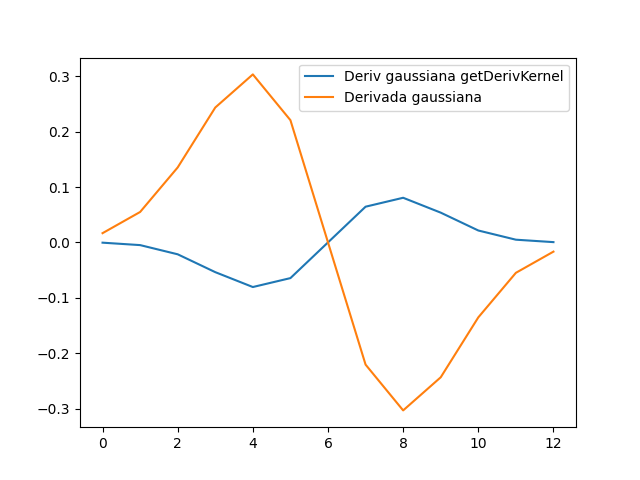
\includegraphics[width=7cm]{images/DerivGaussianaGetDerivKernels.png}
\caption{Máscaras derivadas 1.}
\label{fig:2figsB}
\end{minipage}
\qquad
\begin{minipage}{7cm}
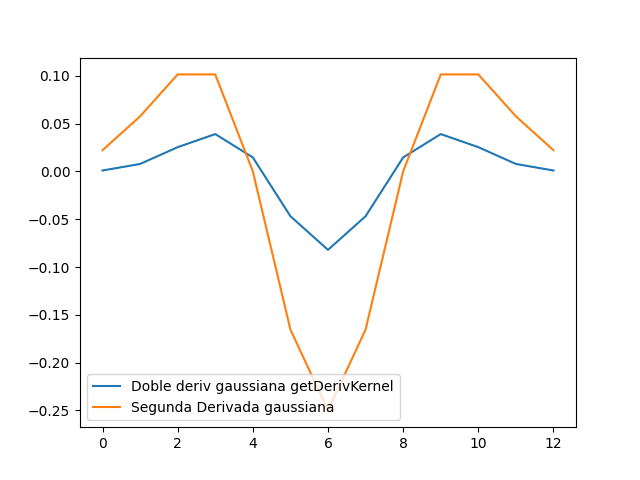
\includegraphics[width=7cm]{images/DobleDerivGaussianaGetDerivKernels.png}
\caption{Máscaras derivadas 2.}
\label{fig:2figsB}
\end{minipage}
\end{figure}
Como mencioné antes, la forma se mantiene pero los valores no.\\
Por último apliqué esas máscaras a la imagen del gato:

\begin{figure}[H]
\centering
\parbox{7cm}{
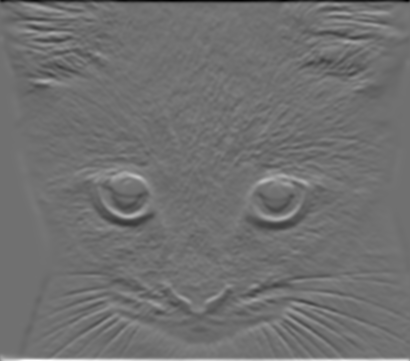
\includegraphics[width=7cm]{images/GetDerivKernelsCat2.png}
\caption{Apliacada máscara sin derivar con $\sigma$=2.}
\label{fig:2figsA}}
\qquad
\begin{minipage}{7cm}
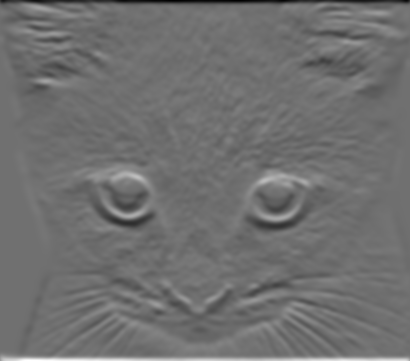
\includegraphics[width=7cm]{images/GetDerivKernelsCat4.png}
\caption{Apliacada máscara sin derivar con $\sigma$=4.}
\label{fig:2figsB}
\end{minipage}
\qquad
\begin{minipage}{7cm}
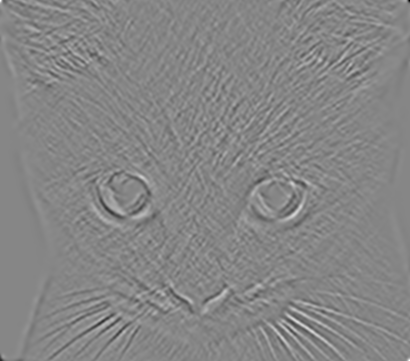
\includegraphics[width=7cm]{images/GetDerivKernelsCatDeriv.png}
\caption{Aplicada máscara derivada con $\sigma$=2.}
\label{fig:2figsB}
\end{minipage}
\qquad
\begin{minipage}{7cm}
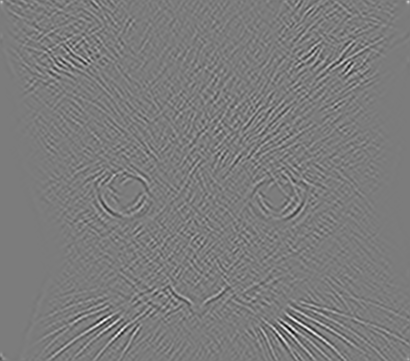
\includegraphics[width=7cm]{images/GetDerivKernelsCatDobleDeriv.png}
\caption{Aplicada máscara doble derivada con $\sigma$=2.}
\label{fig:2figsB}
\end{minipage}
\end{figure}

A pesar de tener valores distintos, el efecto se mantiene pues la forma de la función es muy parecida.

\subsection*{Apartado 1.D}

He creado una función llamada \texttt{laplaciana} para resolver este apartado. Lo que hace es crear cuatro máscaras gaussianas: dos sin derivar y dos derivadas segundas para pasarlas a \texttt{applySeparable2DMask} junto a la imagen y así obtener las imágenes que hay que sumar para terminar de aplicar la máscara laplaciana desada. Esto se obtiene haciendo $\sigma^{2}*(imgx + imgy)$ donde imgx es la imagen resultante de haber aplicado la máscara doble derivada gaussiana en las filas y la sin derivar en columnas y la imgy viceversa (derivada en las filas y sin derivar en las columnas). Para devolver la máscara laplaciana y mostrarla más adelante, he sumado dos matrices llamadas mask1 y mask2: la primera es el resultado de multriplicar la máscara gaussiana doble derivada por otra sin derivar y la segunda matriz viceversa. Las he sumado de la misma forma que las imágenes: $\sigma^{2}*(mask1 + mask2)$.\\\\
En la ejecución y comprobación de este apartado he aplicado las máscaras a la imagen del gato con sigmas 1 y 3 y bordes reflejados y ceros, quedando como resultado el siguiente:

\begin{figure}[H]
\centering
\parbox{5cm}{
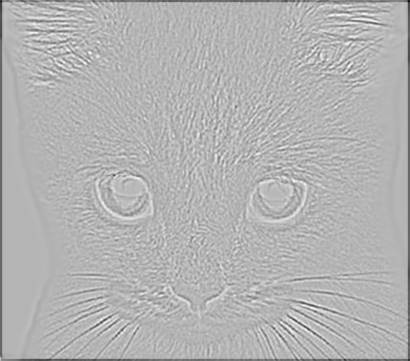
\includegraphics[width=5cm]{images/Lap1cero.png}
\caption{Imagen con $\sigma$=1 y bordes modo cero.}
\label{fig:2figsA}}
\qquad
\begin{minipage}{5cm}
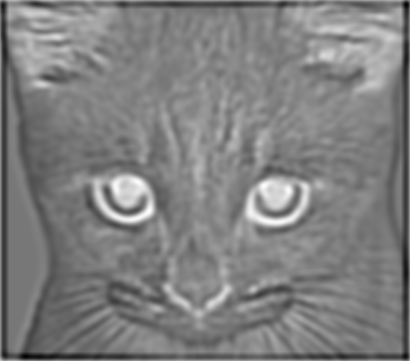
\includegraphics[width=5cm]{images/Lap3cero.png}
\caption{Imagen con $\sigma$=3 y bordes modo cero.}
\label{fig:2figsB}
\end{minipage}
\end{figure}

\begin{figure}[H]
\centering
\parbox{5cm}{
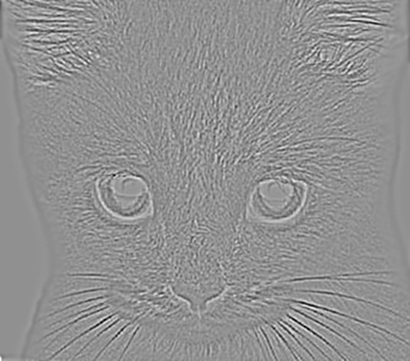
\includegraphics[width=5cm]{images/Lap1reflejo.png}
\caption{Imagen con $\sigma$=1 y bordes modo reflejo.}
\label{fig:2figsA}}
\qquad
\begin{minipage}{5cm}
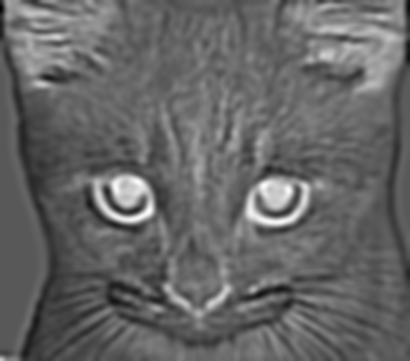
\includegraphics[width=5cm]{images/Lap3reflejo.png}
\caption{Imagen con $\sigma$=3 y bordes modo reflejo.}
\label{fig:2figsB}
\end{minipage}
\end{figure}

Comparando ambos tipos de bordes nos damos cuenta de que el modo de borde que rellena de ceros modifica mucho la imagen y la vuelve algo más blanca que el modo reflejo. Además deja bordes negros en la imagen resultante. Por ello, en general preferiría usar bordes replicados o reflejados.\\
Otro detalle que remarcar en esta comparación es el sigma: cuanto más grande es más se pierden los detalles, como ya íbamos comentando en los anteriores apartados.\\
Por último, las máscaras quedan como sigue:
\begin{figure}[H]
\centering
\parbox{5cm}{

\includegraphics[width=5cm]{images/LapMask1.png}
\caption{Máscara Laplaciana con $\sigma$=1.}
\label{fig:2figsA}}
\qquad
\begin{minipage}{5cm}

\includegraphics[width=5cm]{images/LapMask3.png}
\caption{Máscara Laplaciana con $\sigma$=3.}
\label{fig:2figsB}
\end{minipage}
\end{figure}

\section*{Ejercicio 2}

\subsection*{Apartado 2.A}

En este apartado se pide hacer una pirámide gaussiana, con lo que hay que escribir funciones para reducir el tamaño de las imágenes y aplicar el filtro gaussiano.\\
Para reducir las imágenes he usado el método \texttt{downsampling} que simplemente consiste en eliminar las filas y columnas que estén en las posiciones que son múltiplos de \texttt{ratio}. Es decir, si el ratio es 2, eliminará las filas y columnas que estén en las posiciones 2, 4, 6, 8...\\
Para generar las imágenes de la pirámide, he creado una función llamada \texttt{piramideGaussiana}. Esta función incluye en la pirámide a la imagen original pero no he considerado que ésta entre dentro de los 4 niveles pedidos así que la pirámide tendrá 5 imágenes. El número de niveles se indica con \texttt{nv}, también se debe indicar el sigma y el modo de borde. El parámetro \texttt{ratiods} es el que se le pasará al ratio antes mencionado de \texttt{downsampling}. Lo que hace esta función es aplicar la máscara gaussiana con el sigma que se nos da por parámetro y reducir con \texttt{downsampling} esa imagen (la i-ésima del bucle) devolviendo al final una lista con las imágenes ordenadas de mayor a menor.\\
También he creado una función llamada \texttt{creaImagenPiramide} que crea la imagen de la pirámide vista en teoría a partir de una lista de imágenes \texttt{p} dada por parámetro. Como las imágenes tienen ditintos tamaños, el fondo de la imagen piramidal se mantiene a un color fijo.\\\\
En la ejecución de la pirámide gaussiana he indicado a la función que quiero 4 niveles, con un $\sigma$ = 2, modo de borde replicado (edge) y \texttt{ratiods} por defecto 2 que hará cada imagen que la pirámide a la mitad de tamaño que la anterior. Así, tras obtener la lista resultado donde están las imágenes de la pirámide, se la pasamos a \texttt{creaImagenPiramide} para generar y luego mostrar la imagen piramidal que se vio en teoría. El resultado es el siguiente:

\begin{figure}[H]
\centering
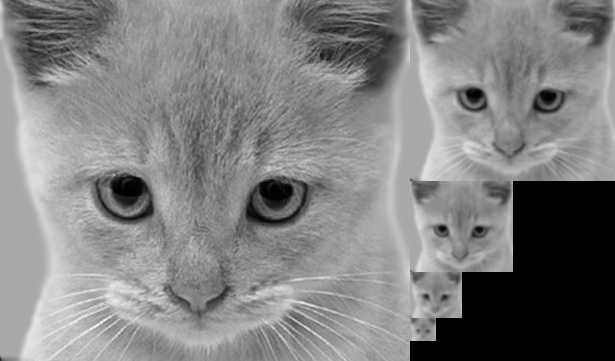
\includegraphics[scale=0.55]{images/PiramideGaussianaGato.png} 
\caption{Pirámide gaussiana de 4 niveles y $\sigma$=2.}
\label{etiqueta}
\end{figure}

Como observación, podemos ver que el modo de borde replicado actúa de forma muy parecida al reflejado: a penas cambia la imagen, a diferencia del modo de borde que rellena de ceros.

\subsection*{Apartado 2.B}

Este apartado pide la creación de una pirámide Laplaciana. Para ello, he creado primero una función para aumentar las imágenes llamada \texttt{upsampling} que repite filas y columnas tantas veces como indica \texttt{ratio}.\\
Para crear la lista de imágenes que formarán la pirámide he definido una función llamada \texttt{piramideLaplaciana} que primero genera la lista de imágenes de la pirámide gaussiana con el mismo número de imágenes y el mismo ratio para el \texttt{downsampling} y como se explica en las diapositivas de teoría, se hace upsampling a la imagen de la pirámide gaussiana y se resta con la de su mismo tamaño, obteniendo así la imagen de la pirámide laplaciana.\\\\
Al igual que en el apartado anterior, he usado bordes replicados, sigma 2, 4 niveles y la imagen del gato y he pasado la lista a la función \texttt{creaImagenPiramide} quedando como resultado el siguiente:

\begin{figure}[H]
\centering
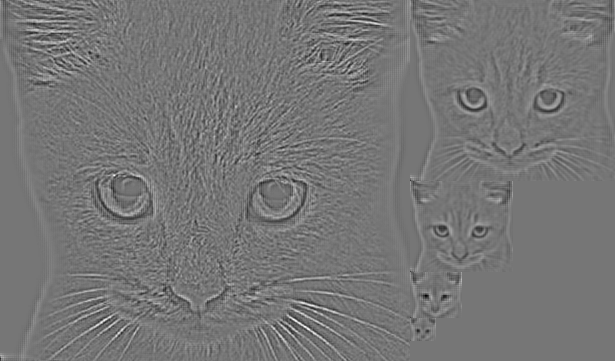
\includegraphics[scale=0.55]{images/PiramideLaplacianaGato.png} 
\caption{Pirámide gaussiana de 4 niveles y $\sigma$=2.}
\label{etiqueta}
\end{figure}

También, para comprobar el buen funcionamiento de esta función he reconstruido la imagen del gato a partir de la última imagen de la pirámide gaussiana mediante el procedimiento inverso, tal y como se explica en teoría, quedando la siguiente imagen:

\begin{figure}[H]
\centering
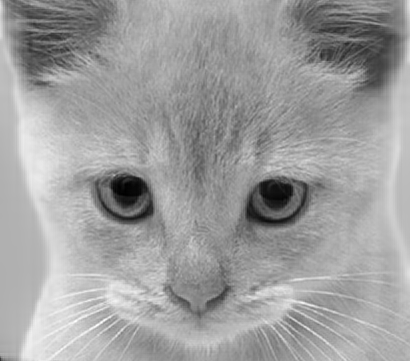
\includegraphics[scale=0.55]{images/GatoReconstruido.png} 
\caption{Pirámide gaussiana de 4 niveles y $\sigma$=2.}
\label{etiqueta}
\end{figure}

\section*{Ejercicio 3}

Para este apartado, como ya introduje al principio, he creado una única función llamada \texttt{ejercicio3} que ejecuta por completo el ejercicio y sus salidas. Lo que hace esta función es leer cada par de imágenes y con ellas llamar a las funciones \texttt{hibridar} y \texttt{creaImagenPiramide} pasándole a esta última la pirámide gaussiana con la imagen híbrida del par de imágenes (devuelta por la función \texttt{hibridar}). Expliquemos ahora lo que hacen estas funciones:\\
\texttt{hibridar} toma como parámetros dos imágenes y dos sigmas: una para paso bajo y otra para paso alto. Para el filtro de paso bajo simplemente se aplica el filtro gaussiano a la imagen y para el de paso alto, será el resultado de restar la imagen original con la imagen con el filtro gaussiano, cada una con su sigma correspondiente. Así la imagen híbrida será el resultado de sumar ambas imágenes, que será devuelta por la función con el nombre de \texttt{imhib}.\\
La función también crea la concatenación de las imágenes normalizadas híbrida, paso alto y paso bajo como pedía el enunciado del ejercicio, mediante la función introducida al principio \texttt{normMatrix} y la devuelve con el nombre de \texttt{res}.\\\\
De este modo, la ejecución de todos los pares de imágenes queda:\\\\\\\\\\\\\\\\\\\\\\
sigma bajo = 8.0\\
sigma alto = 5.0
\begin{figure}[H]
\centering
\parbox{9cm}{
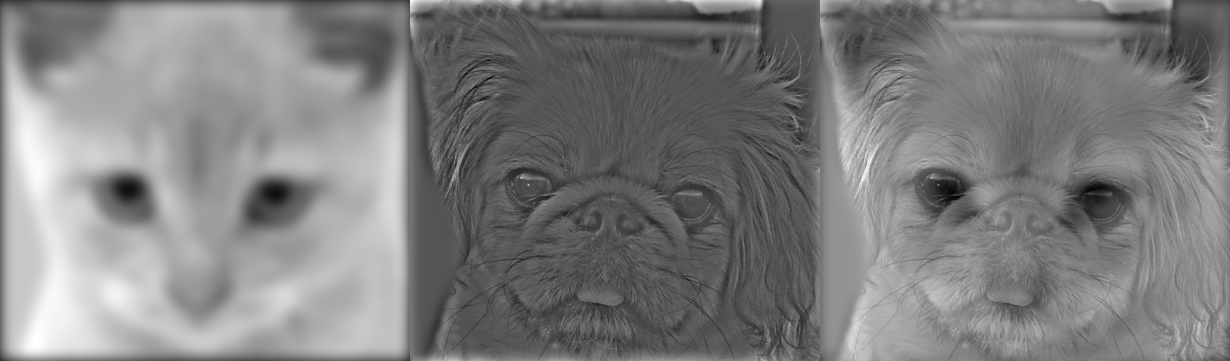
\includegraphics[width=9cm]{images/ImagenGP.png}
\caption{Concatenacion de paso bajo, alto e híbrida para gato y perro.}
\label{fig:2figsA}}
\begin{minipage}{9cm}
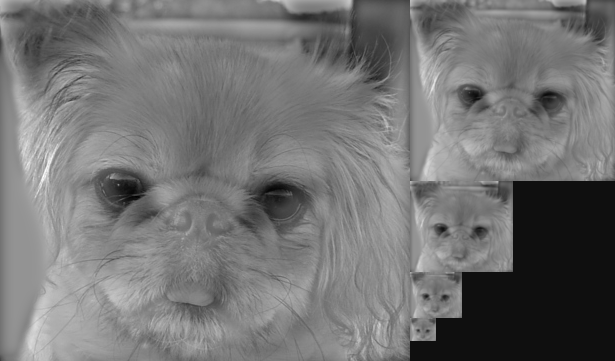
\includegraphics[width=9cm]{images/PirGP.png}
\caption{Pirámide Gaussiana de 4 niveles para gato y perro hibridados.}
\label{fig:2figsB}
\end{minipage}
\end{figure}

sigma alto = 8.0\\
sigma bajo = 3.0
\begin{figure}[H]
\centering
\parbox{9cm}{
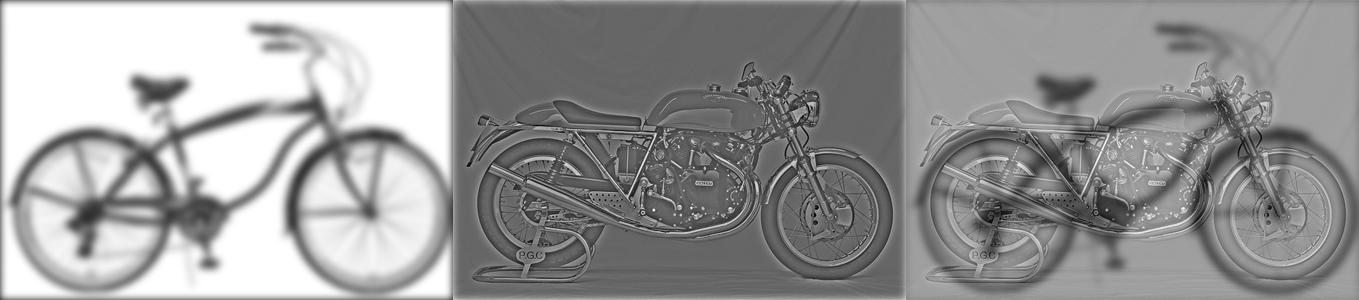
\includegraphics[width=9cm]{images/ImagenMB.png}
\caption{Concatenacion de paso bajo, alto e híbrida para moto y bici.}
\label{fig:2figsA}}
\begin{minipage}{9cm}
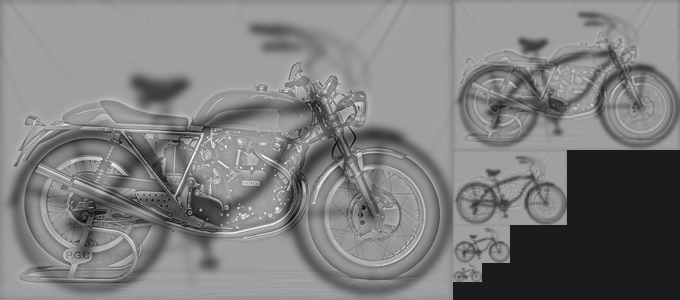
\includegraphics[width=9cm]{images/PirMB.png}
\caption{Pirámide Gaussiana de 4 niveles para moto y bici hibridados.}
\label{fig:2figsB}
\end{minipage}
\end{figure}

sigma bajo = 5.0\\
sigma alto = 2.0
\begin{figure}[H]
\centering
\parbox{9cm}{
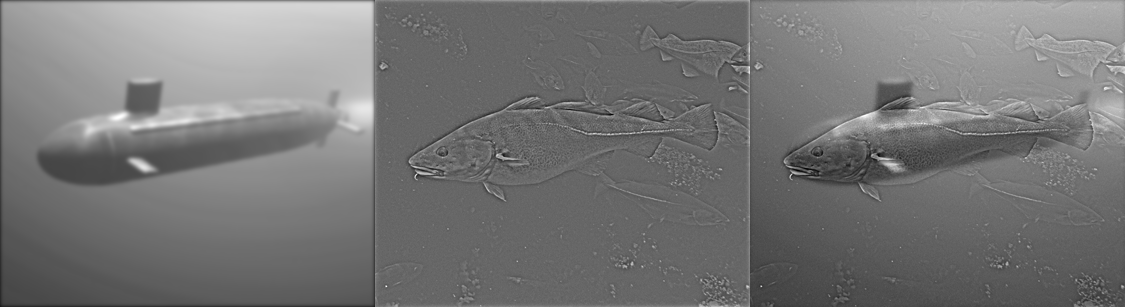
\includegraphics[width=9cm]{images/ImagenPS.png}
\caption{Concatenacion de paso bajo, alto e híbrida para pez y submarino.}
\label{fig:2figsA}}
\begin{minipage}{9cm}
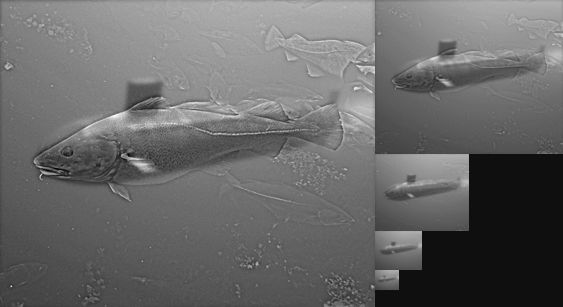
\includegraphics[width=9cm]{images/PirPS.png}
\caption{Pirámide Gaussiana de 4 niveles para pez y submarino hibridados.}
\label{fig:2figsB}
\end{minipage}
\end{figure}

sigma bajo = 6.0\\
sigma alto = 2.0
\begin{figure}[H]
\centering
\parbox{9cm}{
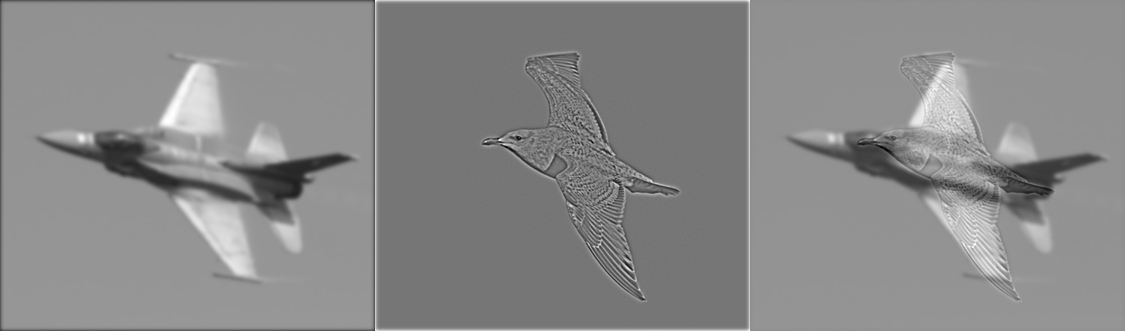
\includegraphics[width=9cm]{images/ImagenPA.png}
\caption{Concatenacion de paso bajo, alto e híbrida para pájaro y avión.}
\label{fig:2figsA}}
\begin{minipage}{9cm}
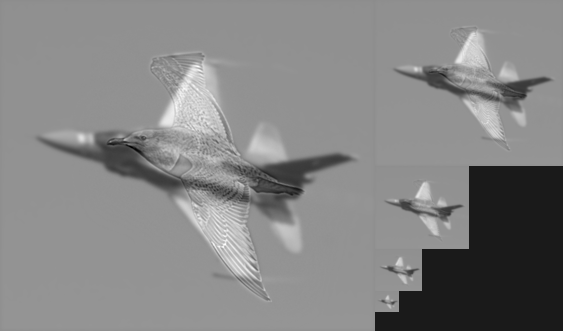
\includegraphics[width=9cm]{images/PirPA.png}
\caption{Pirámide Gaussiana de 4 niveles para pájaro y avión hibridados.}
\label{fig:2figsB}
\end{minipage}
\end{figure}

sigma bajo = 5.0\\
sigma alto = 2.0
\begin{figure}[H]
\centering
\parbox{8cm}{
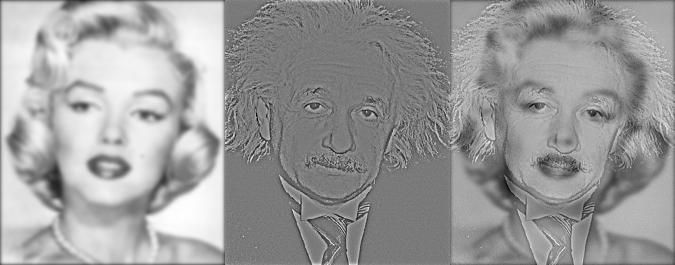
\includegraphics[width=8cm]{images/ImagenEM.png}
\caption{Concatenacion de paso bajo, alto e híbrida para Einstein y Marilyn.}
\label{fig:2figsA}}
\begin{minipage}{8cm}
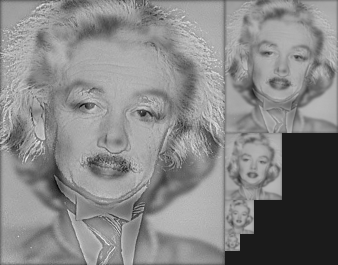
\includegraphics[width=8cm]{images/PirEM.png}
\caption{Pirámide Gaussiana de 4 niveles para Einstein y Marilyn hibridados.}
\label{fig:2figsB}
\end{minipage}
\end{figure}

\section*{Bonus 1}

Para generar las imágenes híbridas en color he hecho lo mismo que en el ejercicio 3 pero leyéndolas en color, pues la función \texttt{hibridar} puede manejar imágenes a color, así como las que crean las piŕamides. De esta forma, he creado las siguientes imágenes híbridas a color, con los mismos sigmas que en ejercicio 3:\\

\begin{figure}[H]
\centering
\parbox{8cm}{
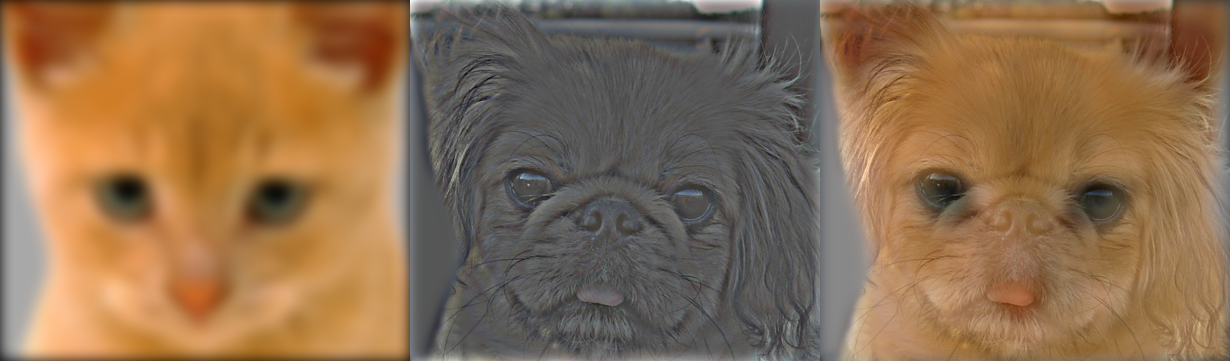
\includegraphics[width=8cm]{images/ImagenGPCol.png}
\caption{Concatenacion de paso bajo, alto e híbrida para gato y perro.}
\label{fig:2figsA}}
\begin{minipage}{8cm}
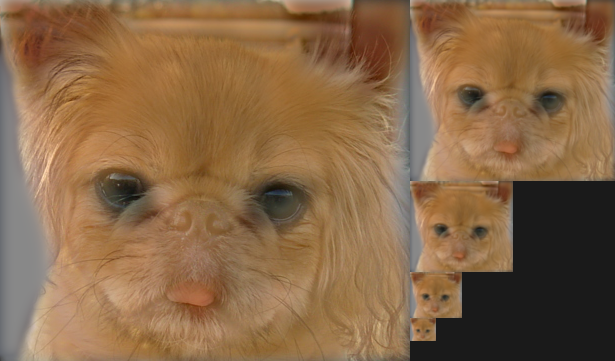
\includegraphics[width=8cm]{images/PirGPCol.png}
\caption{Pirámide Gaussiana de 4 niveles para gato y perro hibridados.}
\label{fig:2figsB}
\end{minipage}
\end{figure}

\begin{figure}[H]
\centering
\parbox{8cm}{
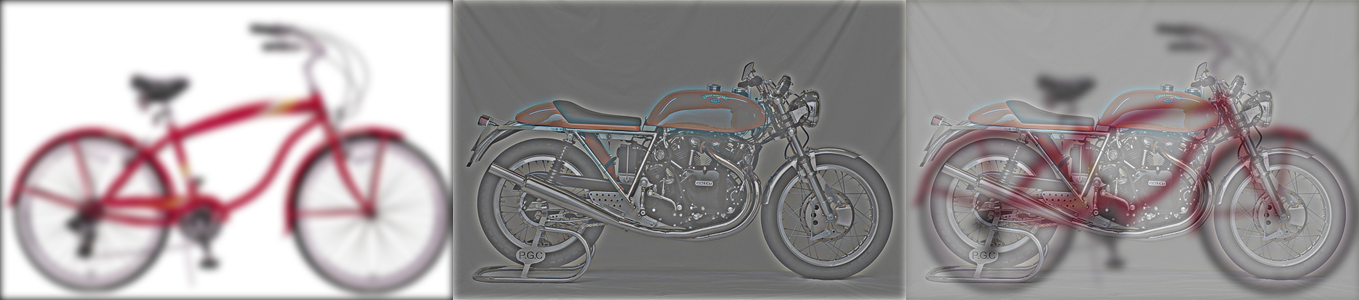
\includegraphics[width=8cm]{images/ImagenMBCol.png}
\caption{Concatenacion de paso bajo, alto e híbrida para moto y bici.}
\label{fig:2figsA}}
\begin{minipage}{8cm}
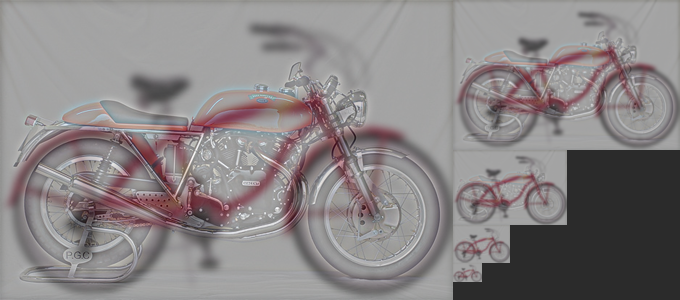
\includegraphics[width=8cm]{images/PirMBCol.png}
\caption{Pirámide Gaussiana de 4 niveles para moto y bici hibridados.}
\label{fig:2figsB}
\end{minipage}
\end{figure}

\begin{figure}[H]
\centering
\parbox{8cm}{
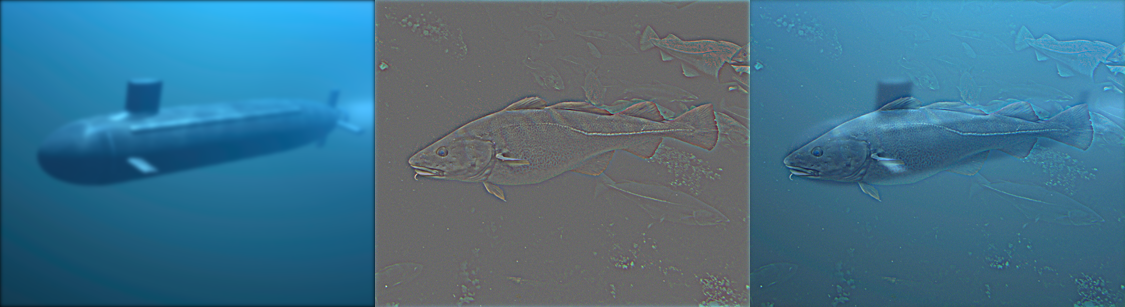
\includegraphics[width=8cm]{images/ImagenPSCol.png}
\caption{Concatenacion de paso bajo, alto e híbrida para pez y submarino.}
\label{fig:2figsA}}
\begin{minipage}{8cm}
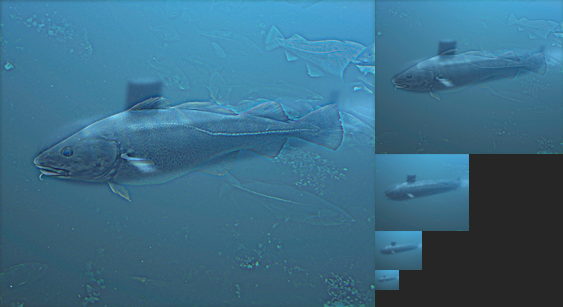
\includegraphics[width=8cm]{images/PirPSCol.png}
\caption{Pirámide Gaussiana de 4 niveles para pez y submarino hibridados.}
\label{fig:2figsB}
\end{minipage}
\end{figure}

\begin{figure}[H]
\centering
\parbox{8cm}{
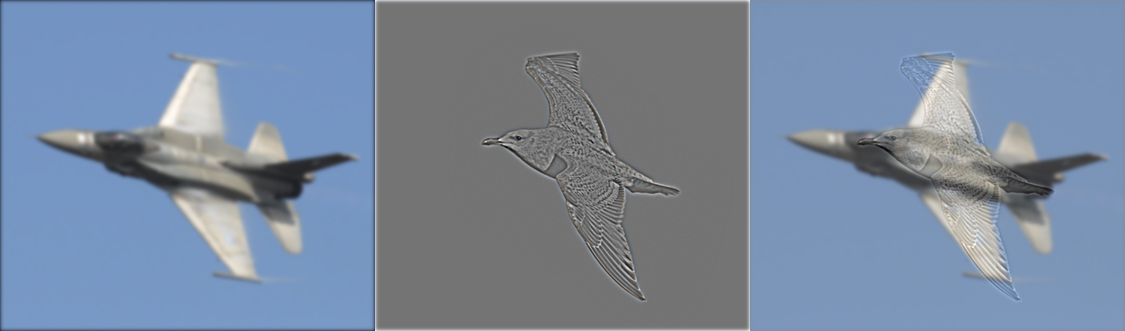
\includegraphics[width=8cm]{images/ImagenPACol.png}
\caption{Concatenacion de paso bajo, alto e híbrida pájaron y avión.}
\label{fig:2figsA}}
\begin{minipage}{8cm}
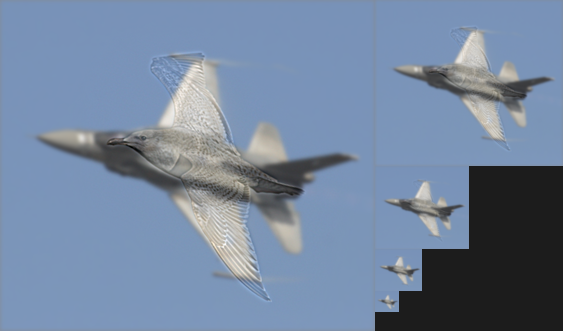
\includegraphics[width=8cm]{images/PirPACol.png}
\caption{Pirámide Gaussiana de 4 niveles para pájaron y avión hibridados.}
\label{fig:2figsB}
\end{minipage}
\end{figure}

\begin{figure}[H]
\centering
\parbox{8cm}{
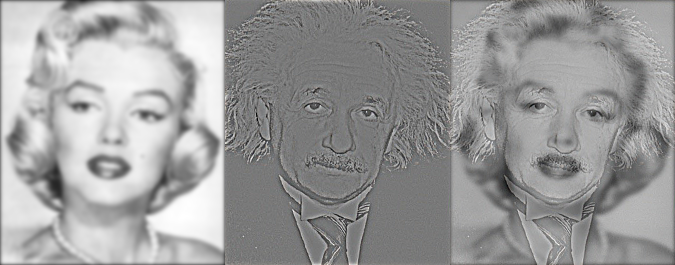
\includegraphics[width=8cm]{images/ImagenEMCol.png}
\caption{Concatenacion de paso bajo, alto e híbrida para Einstein y Marilyn.}
\label{fig:2figsA}}
\begin{minipage}{8cm}
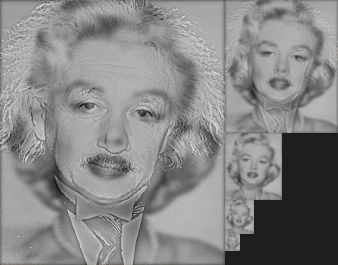
\includegraphics[width=8cm]{images/PirEMCol.png}
\caption{Pirámide Gaussiana de 4 niveles para Einstein y Marilyn hibridados.}
\label{fig:2figsB}
\end{minipage}
\end{figure}

Como observación, el aplicar las máscaras a estas fotos tarda más tiempo de ejecución pues hay que aplicarlas a cada canal de color.

\section*{Bonus 2}

En este caso, había que buscar dos imágenes y crear una híbrida. Lo primero que he hecho ha sido recortar las imágenes de forma que una superpuesta a la otra tengan más o menos la misma silueta para conseguir el efecto.
Después en la función \texttt{bonus2} he seguido los mismos pasos que en el ejercicio 3, aunque esta vez he tenido que hacer \texttt{resize} de openCV para hacer que midieran lo mismo. Así tras hibridarlas con la función \texttt{hibridar} he creado una pirámide y la imagen con las tres: paso alto, paso bajo e híbrida. Las imágenes originales eran:

\begin{figure}[H]
\centering
\parbox{8cm}{
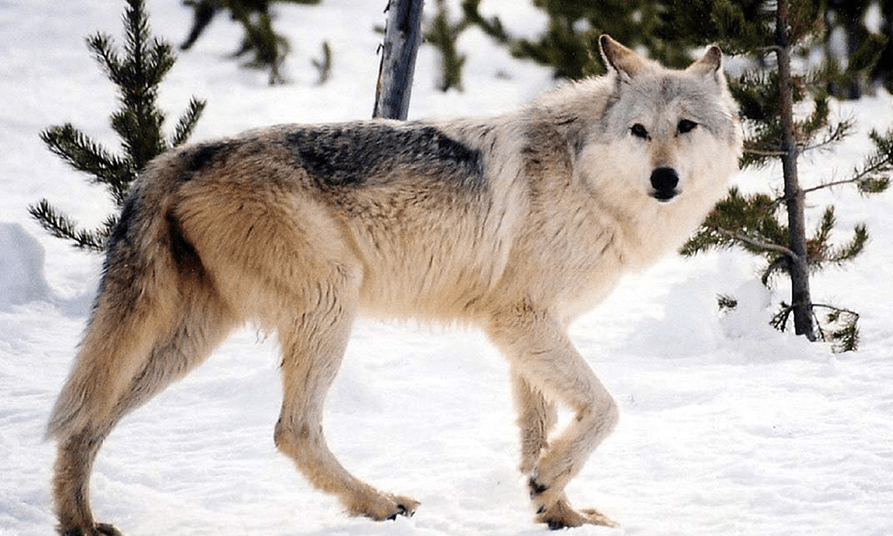
\includegraphics[width=8cm]{images/lobo.png}
\caption{Lobo original.}
\label{fig:2figsA}}
\begin{minipage}{8cm}
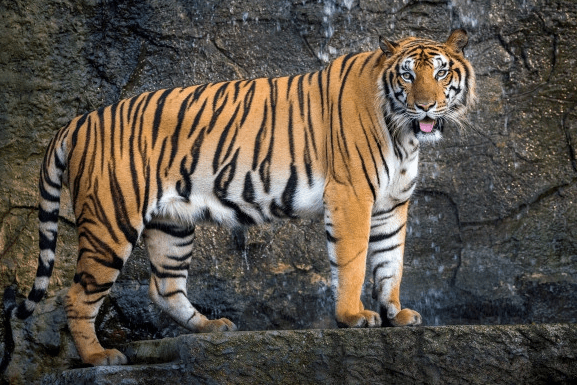
\includegraphics[width=8cm]{images/tigre.png}
\caption{Tigre original.}
\label{fig:2figsB}
\end{minipage}
\end{figure}

Con un sigma bajo de 4.3 y alto de 2.4 el resultado queda:

\begin{figure}[H]
\centering
\parbox{15cm}{
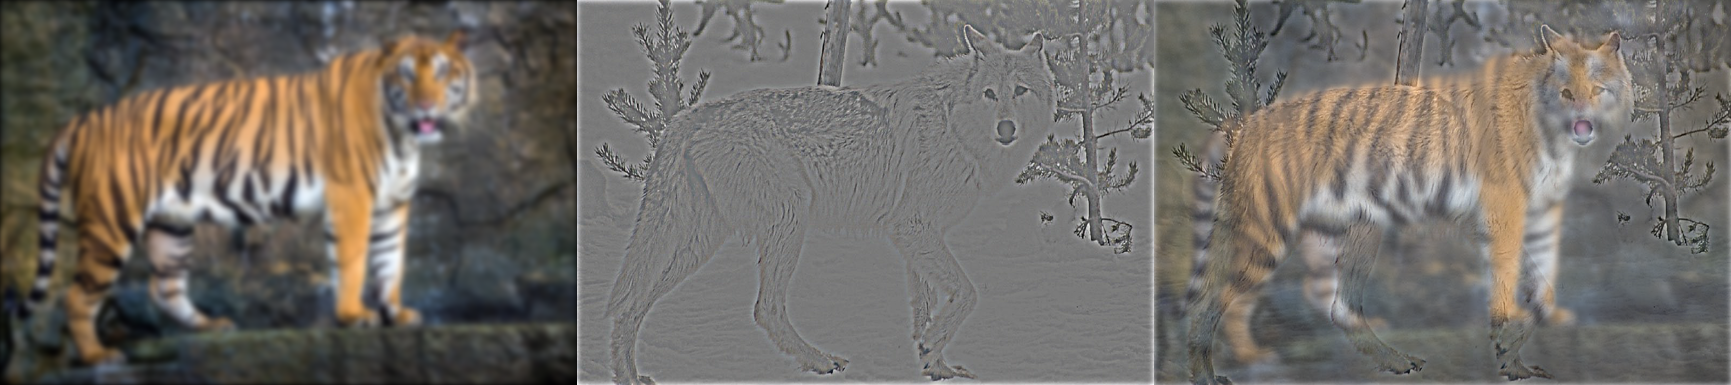
\includegraphics[width=15cm]{images/ImagenLT.png}
\caption{Las tres imágenes juntas.}
\label{fig:2figsA}}
\begin{minipage}{15cm}
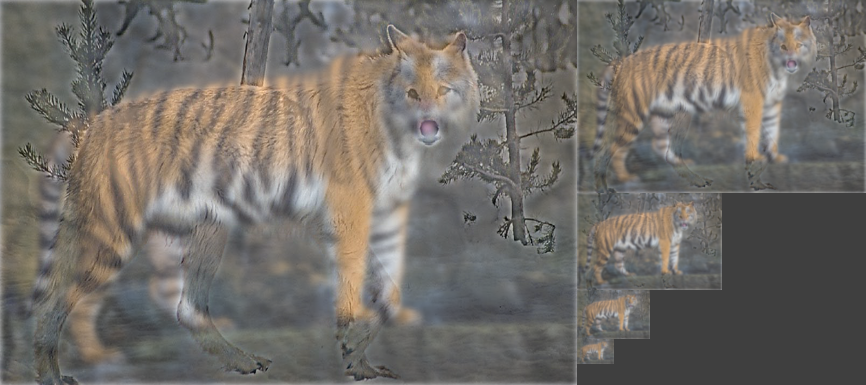
\includegraphics[width=15cm]{images/PirLT.png}
\caption{Prámide gaussiana de 4 niveles con las imágenes hibridadas.}
\label{fig:2figsB}
\end{minipage}
\end{figure}

% --------------------------------------------------------------
%     You don't have to mess with anything below this line.
% --------------------------------------------------------------
 
\end{document}